\documentclass[DIV=14,titlepage=false]{scrreprt}
\usepackage{parskip}
%%%%%%%%%%%%%%%%%%%%%%%%%%%%%%%%%%%%%%%%%%%%%%%%%%%%%%%%%%%%%%%%%%%%%%%%%%%%%%%
%                                Basic Packages                               %
%%%%%%%%%%%%%%%%%%%%%%%%%%%%%%%%%%%%%%%%%%%%%%%%%%%%%%%%%%%%%%%%%%%%%%%%%%%%%%%
% Gives us multiple colors.
\usepackage[usenames,dvipsnames,pdftex]{xcolor}
% Lets us style link colors.
\usepackage{hyperref}
% Lets us import images and graphics.
\usepackage{graphicx}
% Lets us use figures in floating environments.
\usepackage{float}
% Lets us create multiple columns.
\usepackage{multicol}
% Gives us better math syntax.
\usepackage{amsmath,amsfonts,mathtools,amsthm,amssymb}
% Lets us strikethrough text.
\usepackage{cancel}
% Lets us edit the caption of a figure.
\usepackage{caption}
% Lets us import pdf directly in our tex code.
\usepackage{pdfpages}
% Lets us do algorithm stuff.
\usepackage[ruled,vlined,linesnumbered]{algorithm2e}
% Gets rid of some errors.
\usepackage{scrhack}
\def\class{article}
\usepackage{geometry}
\geometry{margin=0.9in}
%%%%%%%%%%%%%%%%%%%%%%%%%%%%%%%%%%%%%%%%%%%%%%%%%%%%%%%%%%%%%%%%%%%%%%%%%%%%%%%
%                                Basic Settings                               %
%%%%%%%%%%%%%%%%%%%%%%%%%%%%%%%%%%%%%%%%%%%%%%%%%%%%%%%%%%%%%%%%%%%%%%%%%%%%%%%

%%%%%%%%%%%%%
%  Symbols  %
%%%%%%%%%%%%%

\let\implies\Rightarrow
\let\impliedby\Leftarrow
\let\iff\Leftrightarrow
\let\epsilon\varepsilon

%%%%%%%%%%%%
%  Tables  %
%%%%%%%%%%%%

\setlength{\tabcolsep}{5pt}
\renewcommand\arraystretch{1.5}

%%%%%%%%%%%%%%%%%%%%%%%
%  Center Title Page  %
%%%%%%%%%%%%%%%%%%%%%%%

\usepackage{titling}
\renewcommand\maketitlehooka{\null\mbox{}\vfill}
\renewcommand\maketitlehookd{\vfill\null}

%%%%%%%%%%%%%%%%%%%%%%%%%%%%%%%%%%%%%%%%%%%%%%%%%%%%%%%
%  Create a grey background in the middle of the PDF  %
%%%%%%%%%%%%%%%%%%%%%%%%%%%%%%%%%%%%%%%%%%%%%%%%%%%%%%%

\usepackage{eso-pic}
\newcommand\definegraybackground{
  \definecolor{reallylightgray}{HTML}{FAFAFA}
  \AddToShipoutPicture{
    \ifthenelse{\isodd{\thepage}}{
      \AtPageLowerLeft{
        \put(\LenToUnit{\dimexpr\paperwidth-222pt},0){
          \color{reallylightgray}\rule{222pt}{297mm}
        }
      }
    }
    {
      \AtPageLowerLeft{
        \color{reallylightgray}\rule{222pt}{297mm}
      }
    }
  }
}

%%%%%%%%%%%%%%%%%%%%%%%%
%  Modify Links Color  %
%%%%%%%%%%%%%%%%%%%%%%%%

\hypersetup{
  % Enable highlighting links.
  colorlinks,
  % Change the color of links to blue.
  linkcolor={black},
  % Change the color of citations to black.
  citecolor={black},
  % Change the color of url's to blue with some black.
  urlcolor=blue
}

%%%%%%%%%%%%%%%%%%
% Fix WrapFigure %
%%%%%%%%%%%%%%%%%%

\newcommand{\wrapfill}{\par\ifnum\value{WF@wrappedlines}>0
    \parskip=0pt
    \addtocounter{WF@wrappedlines}{-1}%
    \null\vspace{\arabic{WF@wrappedlines}\baselineskip}%
    \WFclear
\fi}

%%%%%%%%%%%%%%%%%
% Multi Columns %
%%%%%%%%%%%%%%%%%

\let\multicolmulticols\multicols
\let\endmulticolmulticols\endmulticols

\RenewDocumentEnvironment{multicols}{mO{}}
{%
  \ifnum#1=1
    #2%
  \else % More than 1 column
    \multicolmulticols{#1}[#2]
  \fi
}
{%
  \ifnum#1=1
\else % More than 1 column
  \endmulticolmulticols
\fi
}

\newlength{\thickarrayrulewidth}
\setlength{\thickarrayrulewidth}{5\arrayrulewidth}

%%%%%%%%%%%%%%%%%%%%
%  Import Figures  %
%%%%%%%%%%%%%%%%%%%%

\usepackage{import}
\pdfminorversion=7

% EXAMPLE:
% 1. \incfig{limit-graph}
% 2. \incfig[0.4]{limit-graph}
% Parameters:
% 1. The figure name. It should be located in figures/NAME.tex_pdf.
% 2. (Optional) The width of the figure. Example: 0.5, 0.35.
\newcommand\incfig[2][1]{%
  \def\svgwidth{#1\columnwidth}
  \import{./figures/}{#2.pdf_tex}
}

\begingroup\expandafter\expandafter\expandafter\endgroup
\expandafter\ifx\csname pdfsuppresswarningpagegroup\endcsname\relax
\else
  \pdfsuppresswarningpagegroup=1\relax
\fi

%%%%%%%%%%%%%
%  Correct  %
%%%%%%%%%%%%%

% EXAMPLE:
% 1. \correct{INCORRECT}{CORRECT}
% Parameters:
% 1. The incorrect statement.
% 2. The correct statement.
\definecolor{correct}{HTML}{009900}
\newcommand\correct[2]{{\color{red}{#1 }}\ensuremath{\to}{\color{correct}{ #2}}}



\newcommand{\R}{\mathbb{R}}
\newcommand{\Z}{\mathbb{Z}}
\newcommand{\E}{\mathbb{E}}
\newcommand{\B}{\ensuremath{\mathcal{B}}}
\newcommand{\X}{\ensuremath{\mathcal{X}}}
\newcommand{\Y}{\ensuremath{\mathcal{Y}}}
\newcommand{\mA}{\ensuremath{\mathbf{A}}}
\newcommand{\mB}{\ensuremath{\mathbf{B}}}
\newcommand{\mC}{\ensuremath{\mathbf{C}}}
\newcommand{\mD}{\ensuremath{\mathbf{D}}}
\newcommand{\mX}{\ensuremath{\mathbf{X}}}
\newcommand{\mY}{\ensuremath{\mathbf{Y}}}
\newcommand{\mx}{\ensuremath{\mathbf{x}}}
\newcommand{\my}{\ensuremath{\mathbf{y}}}
\newcommand{\mI}{\ensuremath{\mathbf{I}}}
\newcommand{\mi}{\ensuremath{\mathbf{\iota}}}
\newcommand{\mmu}{\ensuremath{\mathbf{\mu}}}
\newcommand{\mc}{\ensuremath{\mathbf{c}}}
\newcommand{\mSigma}{\ensuremath{\mathbf{\Sigma}}}
\newcommand{\mzero}{\ensuremath{\mathbf{0}}}
\newcommand{\independent}{\perp\!\!\!\!\perp} 
\setlength{\parindent}{0pt}
%%%%%%%%%%%%%%%%%%%%%%%%%%%%%%%%%%%%%%%%%%%%%%%%%%%%%%%%%%%%%%%%%%%%%%%%%%%%%%%
%                                 Environments                                %
%%%%%%%%%%%%%%%%%%%%%%%%%%%%%%%%%%%%%%%%%%%%%%%%%%%%%%%%%%%%%%%%%%%%%%%%%%%%%%%

\usepackage{varwidth}
\usepackage{thmtools}
\usepackage[most,many,breakable]{tcolorbox}

\tcbuselibrary{theorems,skins,hooks}
\usetikzlibrary{arrows,calc,shadows.blur}

%%%%%%%%%%%%%%%%%%%
%  Define Colors  %
%%%%%%%%%%%%%%%%%%%

\definecolor{myblue}{RGB}{45, 111, 177}
\definecolor{mygreen}{RGB}{56, 140, 70}
\definecolor{myred}{RGB}{199, 68, 64}
\definecolor{mypurple}{RGB}{197, 92, 212}

\definecolor{definition}{HTML}{228b22}
\definecolor{theorem}{HTML}{00007B}
\definecolor{example}{HTML}{2A7F7F}
\definecolor{definition}{HTML}{228b22}
\definecolor{prop}{HTML}{191971}
\definecolor{lemma}{HTML}{983b0f}
\definecolor{exercise}{HTML}{88D6D1}

\colorlet{definition}{mygreen!85!black}
\colorlet{claim}{mygreen!85!black}
\colorlet{corollary}{mypurple!85!black}
\colorlet{proof}{theorem}

%%%%%%%%%%%%%%%%%%%%%%
%  Helpful Commands  %
%%%%%%%%%%%%%%%%%%%%%%

% EXAMPLE:
% 1. \createnewtheoremstyle{thmdefinitionbox}{}{}
% 2. \createnewtheoremstyle{thmtheorembox}{}{}
% 3. \createnewtheoremstyle{thmproofbox}{qed=\qedsymbol}{
%       rightline=false, topline=false, bottomline=false
%    }
% Parameters:
% 1. Theorem name.
% 2. Any extra parameters to pass directly to declaretheoremstyle.
% 3. Any extra parameters to pass directly to mdframed.
\newcommand\createnewtheoremstyle[3]{
  \declaretheoremstyle[
  headfont=\bfseries\sffamily, bodyfont=\normalfont, #2,
  mdframed={
    #3,
  },
  ]{#1}
}

% EXAMPLE:
% 1. \createnewcoloredtheoremstyle{thmdefinitionbox}{definition}{}{}
% 2. \createnewcoloredtheoremstyle{thmexamplebox}{example}{}{
%       rightline=true, leftline=true, topline=true, bottomline=true
%     }
% 3. \createnewcoloredtheoremstyle{thmproofbox}{proof}{qed=\qedsymbol}{backgroundcolor=white}
% Parameters:
% 1. Theorem name.
% 2. Color of theorem.
% 3. Any extra parameters to pass directly to declaretheoremstyle.
% 4. Any extra parameters to pass directly to mdframed.
\newcommand\createnewcoloredtheoremstyle[4]{
  \declaretheoremstyle[
  headfont=\bfseries\sffamily\color{#2}, bodyfont=\normalfont, #3,
  mdframed={
    linewidth=2pt,
    rightline=false, leftline=true, topline=false, bottomline=false,
    linecolor=#2, backgroundcolor=#2!5, #4,
  },
  ]{#1}
}

%%%%%%%%%%%%%%%%%%%%%%%%%%%%%%%%%%%
%  Create the Environment Styles  %
%%%%%%%%%%%%%%%%%%%%%%%%%%%%%%%%%%%

\makeatletter
\@ifclasswith\class{nocolor}{
  % Environments without color.

  \createnewtheoremstyle{thmdefinitionbox}{}{}
  \createnewtheoremstyle{thmtheorembox}{}{}
  \createnewtheoremstyle{thmexamplebox}{}{}
  \createnewtheoremstyle{thmclaimbox}{}{}
  \createnewtheoremstyle{thmcorollarybox}{}{}
  \createnewtheoremstyle{thmpropbox}{}{}
  \createnewtheoremstyle{thmlemmabox}{}{}
  \createnewtheoremstyle{thmexercisebox}{}{}
  \createnewtheoremstyle{thmdefinitionbox}{}{}
  \createnewtheoremstyle{thmquestionbox}{}{}
  \createnewtheoremstyle{thmsolutionbox}{}{}

  \createnewtheoremstyle{thmproofbox}{qed=\qedsymbol}{}
  \createnewtheoremstyle{thmexplanationbox}{}{}
}{
  % Environments with color.

  \createnewcoloredtheoremstyle{thmdefinitionbox}{definition}{}{}
  \createnewcoloredtheoremstyle{thmtheorembox}{theorem}{}{}
  \createnewcoloredtheoremstyle{thmexamplebox}{example}{}{
    rightline=true, leftline=true, topline=true, bottomline=true
  }
  \createnewcoloredtheoremstyle{thmclaimbox}{claim}{}{}
  \createnewcoloredtheoremstyle{thmcorollarybox}{corollary}{}{}
  \createnewcoloredtheoremstyle{thmpropbox}{prop}{}{}
  \createnewcoloredtheoremstyle{thmlemmabox}{lemma}{}{}
  \createnewcoloredtheoremstyle{thmexercisebox}{exercise}{}{}

  \createnewcoloredtheoremstyle{thmproofbox}{proof}{qed=\qedsymbol}{backgroundcolor=white}
  \createnewcoloredtheoremstyle{thmexplanationbox}{example}{qed=\qedsymbol}{backgroundcolor=white}
}
\makeatother

%%%%%%%%%%%%%%%%%%%%%%%%%%%%%
%  Create the Environments  %
%%%%%%%%%%%%%%%%%%%%%%%%%%%%%

\declaretheorem[numberwithin=section, style=thmtheorembox,     name=Theorem]{theorem}
\declaretheorem[numbered=no,          style=thmexamplebox,     name=Example]{example}
\declaretheorem[numberwithin=section, style=thmclaimbox,       name=Claim]{claim}
\declaretheorem[numberwithin=section, style=thmcorollarybox,   name=Corollary]{corollary}
\declaretheorem[numberwithin=section, style=thmpropbox,        name=Proposition]{prop}
\declaretheorem[numberwithin=section, style=thmlemmabox,       name=Lemma]{lemma}
\declaretheorem[numberwithin=section, style=thmexercisebox,    name=Exercise]{exercise}
\declaretheorem[numbered=no,          style=thmproofbox,       name=Proof]{replacementproof}
\declaretheorem[numbered=no,          style=thmexplanationbox, name=Proof]{expl}

\makeatletter
\@ifclasswith\class{nocolor}{
  % Environments without color.

  \newtheorem*{note}{Note}

  \declaretheorem[numberwithin=section, style=thmdefinitionbox, name=Definition]{definition}
  \declaretheorem[numberwithin=section, style=thmquestionbox,   name=Question]{question}
  \declaretheorem[numberwithin=section, style=thmsolutionbox,   name=Solution]{solution}
}{
  % Environments with color.

  \newtcbtheorem[number within=section]{Definition}{Definition}{
    enhanced,
    before skip=2mm,
    after skip=2mm,
    colback=red!5,
    colframe=red!80!black,
    colbacktitle=red!75!black,
    boxrule=0.5mm,
    attach boxed title to top left={
      xshift=1cm,
      yshift*=1mm-\tcboxedtitleheight
    },
    varwidth boxed title*=-3cm,
    boxed title style={
      interior engine=empty,
      frame code={
        \path[fill=tcbcolback]
        ([yshift=-1mm,xshift=-1mm]frame.north west)
        arc[start angle=0,end angle=180,radius=1mm]
        ([yshift=-1mm,xshift=1mm]frame.north east)
        arc[start angle=180,end angle=0,radius=1mm];
        \path[left color=tcbcolback!60!black,right color=tcbcolback!60!black,
        middle color=tcbcolback!80!black]
        ([xshift=-2mm]frame.north west) -- ([xshift=2mm]frame.north east)
        [rounded corners=1mm]-- ([xshift=1mm,yshift=-1mm]frame.north east)
        -- (frame.south east) -- (frame.south west)
        -- ([xshift=-1mm,yshift=-1mm]frame.north west)
        [sharp corners]-- cycle;
      },
    },
    fonttitle=\bfseries,
    title={#2},
    #1
  }{def}

  \NewDocumentEnvironment{definition}{O{}O{}}
    {\begin{Definition}{#1}{#2}}{\end{Definition}}

  \newtcolorbox{note}[1][]{%
    enhanced jigsaw,
    colback=gray!20!white,%
    colframe=gray!80!black,
    size=small,
    boxrule=1pt,
    title=\textbf{Note:-},
    halign title=flush center,
    coltitle=black,
    breakable,
    drop shadow=black!50!white,
    attach boxed title to top left={xshift=1cm,yshift=-\tcboxedtitleheight/2,yshifttext=-\tcboxedtitleheight/2},
    minipage boxed title=1.5cm,
    boxed title style={%
      colback=white,
      size=fbox,
      boxrule=1pt,
      boxsep=2pt,
      underlay={%
        \coordinate (dotA) at ($(interior.west) + (-0.5pt,0)$);
        \coordinate (dotB) at ($(interior.east) + (0.5pt,0)$);
        \begin{scope}
          \clip (interior.north west) rectangle ([xshift=3ex]interior.east);
          \filldraw [white, blur shadow={shadow opacity=60, shadow yshift=-.75ex}, rounded corners=2pt] (interior.north west) rectangle (interior.south east);
        \end{scope}
        \begin{scope}[gray!80!black]
          \fill (dotA) circle (2pt);
          \fill (dotB) circle (2pt);
        \end{scope}
      },
    },
    #1,
  }

  \newtcbtheorem{Question}{Question}{enhanced,
    breakable,
    colback=white,
    colframe=myblue!80!black,
    attach boxed title to top left={yshift*=-\tcboxedtitleheight},
    fonttitle=\bfseries,
    title=\textbf{Question:-},
    boxed title size=title,
    boxed title style={%
      sharp corners,
      rounded corners=northwest,
      colback=tcbcolframe,
      boxrule=0pt,
    },
    underlay boxed title={%
      \path[fill=tcbcolframe] (title.south west)--(title.south east)
      to[out=0, in=180] ([xshift=5mm]title.east)--
      (title.center-|frame.east)
      [rounded corners=\kvtcb@arc] |-
      (frame.north) -| cycle;
    },
    #1
  }{def}

  \NewDocumentEnvironment{question}{O{}O{}}
  {\begin{Question}{#1}{#2}}{\end{Question}}

  \newtcolorbox{Solution}{enhanced,
    breakable,
    colback=white,
    colframe=mygreen!80!black,
    attach boxed title to top left={yshift*=-\tcboxedtitleheight},
    title=\textbf{Solution:-},
    boxed title size=title,
    boxed title style={%
      sharp corners,
      rounded corners=northwest,
      colback=tcbcolframe,
      boxrule=0pt,
    },
    underlay boxed title={%
      \path[fill=tcbcolframe] (title.south west)--(title.south east)
      to[out=0, in=180] ([xshift=5mm]title.east)--
      (title.center-|frame.east)
      [rounded corners=\kvtcb@arc] |-
      (frame.north) -| cycle;
    },
  }

  \NewDocumentEnvironment{solution}{O{}O{}}
  {\vspace{-10pt}\begin{Solution}{#1}{#2}}{\end{Solution}}
}
\makeatother

%%%%%%%%%%%%%%%%%%%%%%%%%%%%
%  Edit Proof Environment  %
%%%%%%%%%%%%%%%%%%%%%%%%%%%%

\renewenvironment{proof}[1][\proofname]{\vspace{-10pt}\begin{replacementproof}}{\end{replacementproof}}
\newenvironment{explanation}[1][\proofname]{\vspace{-10pt}\begin{expl}}{\end{expl}}

\theoremstyle{definition}

\newtheorem*{notation}{Notation}
\newtheorem*{previouslyseen}{As previously seen}
\newtheorem*{problem}{Problem}
\newtheorem*{observe}{Observe}
\newtheorem*{property}{Property}
\newtheorem*{intuition}{Intuition}

\title{%
R300 Econometrics}
\author{Metrics Enjoyers}
\date{Michaelmas Term, 2023-2024}

\setuptoc{toc}{leveldown}
\setcounter{chapter}{2}

\begin{document}
\pagenumbering{gobble}
\chapter{Geometric Interpretation of OLS, Mean Variance of OLS, Partitioned Regression}
\section{Geometric Interpretation}
Consider estimation of \(\beta\) in the model:
\[y_{i}=x^{'}_{i}\beta + \epsilon_{i}, \ i=1,...,n\]
This is equivalent in matrix form to: \(Y=X\beta+\epsilon\)

The OLS estimator is: \(\hat{\beta}=(X^{'}X)^{-1}X^{'}Y\)
\begin{definition}
  The \underline{\smash{Projection Matrix}} is defined as: \[P_X=X(X^{'}X)^{-1}X^{'}\]
  The \underline{Residual Maker Matrix} is defined as: \[M_X=I-P_X\]
\end{definition}

Then \[\hat{Y}=X\hat{\beta}=P_XY\] \[\hat{\epsilon}=Y-\hat{Y}=M_XY\]

\begin{claim}
  \(P_X\) and \(M_X\) are symmetric and idempotent.
\end{claim}

\begin{center}
  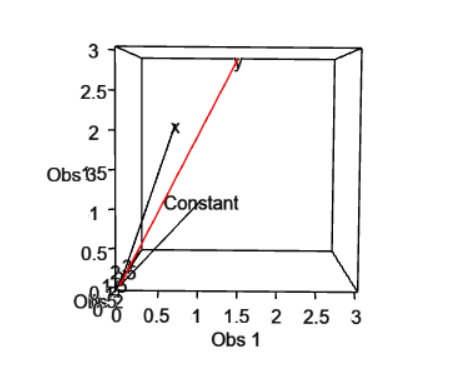
\includegraphics[width=0.5\textwidth]{./Images/OLS as projection.png}
\end{center}

Thus, \(\hat{Y}=X\hat{\beta}\) is the orthogonal projection of the n-dimensional vector \(Y\) onto the subspace spanned by the columns of \(X\).
Each column of X represents the n values that each regressor takes for every observation. 

The "subspace" spanned by the columns of \(X\) is the set of all linear combinations of the columns of \(X\). The orthogonal projection of \(Y\) onto this subspace is the closest point in the subspace to \(Y\). This is because we solve:

\[\hat{\beta} = \operatorname*{argmin}_{b} \sum(y_i-x'_ib)^2 = \operatorname*{argmin}_{b} (Y-Xb)^{'}(Y-Xb)=\operatorname*{argmin}_{b}\|Y-Xb\|^2\]

\begin{example}
  \(k=n\)

  Clearly if we had k=n regressors, then the columns of \(X\) would span the entire n-dimensional space and the projection would be the identity matrix. In this case, \(\hat{Y}=Y\), and the residuals would be zero.
\end{example}

\subsection{The Residual Vector}

The difference between \(Y\) and the projection of \(Y\) onto the subspace is the residual vector \(\hat{\epsilon}\). 

\vspace{5mm}

\begin{claim}
  The residual vector is orthogonal to the subspace spanned by the columns of \(X\) and so is orthogonal to each column of \(X\) \(X'\hat{\epsilon}=0\)
\end{claim}

\vspace{5mm}

\begin{proof}
  Intuitively:
  This is because the projection of \(Y\) onto the subspace is the closest point in the subspace to \(Y\). If the residual vector were not orthogonal to the subspace, then we could move the projection of \(Y\) onto the subspace along the residual vector and get a point that is closer to \(Y\). This would contradict the fact that the projection of \(Y\) onto the subspace is the closest point in the subspace to \(Y\).

  Algebraically:
  \[X'\hat{\epsilon}=X'(Y-\hat{Y})=X'(Y-P_XY)=X'(Y-X(X'X)^{-1}X'Y)=0\]

\end{proof}
 
\section{Conditional Mean and Variance of OLS}

\subsection{Conditional Mean}

\begin{claim}
  \(\hat{\beta}\) is a conditionally unbiased estimator of \(\beta\) \[\mathbb{E}[\hat{\beta}|X]=\beta\]
\end{claim}

\vspace{5mm}

\begin{proof}
  \[\hat{\beta}=(X'X)^{-1}X'Y = (X'X)^{-1}X'(X\beta+\epsilon)=\beta+(X'X)^{-1}X'\epsilon\]
  \[\mathbb{E}[\hat{\beta}|X]=\beta+(X'X)^{-1}X'\mathbb{E}[\epsilon|X]\operatorname*{=}^1\beta \] 
  \begin{center}
    1. via strict exogeneity \(\mathbb{E}[\epsilon|X]=0\), do not need iid (e.g. can have a regressor \(x_i=i\))
  \end{center}
\end{proof}

Also only need strict exogeneity for a causal interpretation of \(\beta\).

\vspace{5mm}

\begin{claim}
  \(\hat{\beta}\) is an unconditionally unbiased estimator of \(\beta\), provided expectations exist \[\mathbb{E}[\hat{\beta}|X]=\beta\]
\end{claim}

\vspace{5mm}

\begin{proof} via law of iterated expectations
  \[\mathbb{E}[\hat{\beta}]=\mathbb{E}[\mathbb{E}[\hat{\beta}|X]]=\mathbb{E}[\beta]=\beta\]
\end{proof}

\subsection{Conditional Variance}

\vspace{5mm}

\begin{theorem}
  \[Var(\hat{\beta}|X)=\sigma^2(X'X)^{-1}\]
\end{theorem}

\vspace{5mm}

%\begin{proof}
  
\vspace{5mm}

\begin{lemma} Unconditional Variance of a vector:
  \[Var(z)=\mathbb{E}[(z-\mathbb{E}[z])(z-\mathbb{E}[z])']=\mathbb{E}[zz']-\mathbb{E}[z]\mathbb{E}[z']\]
\end{lemma}

\begin{corollary} 
Conditional Variance of a vector:
\[Var(z|X)=\mathbb{E}[zz'|X]-\mathbb{E}[z|X]\mathbb{E}[z'|X]\]
\end{corollary}

Thus for \(z = A(X)w\) where A is a matrix that depends on X we have:
\[Var(z|X)= \mathbb{{E}}[A(X)w w' A(X)'|X]-\mathbb{{E}}[A(X)w|X]\mathbb{{E}}[w' A(X)'|X]\]
\[=A(X)\mathbb{E}[ww'|X]A(X)'-A(X)\mathbb{E}[w|X]\mathbb{E}[w'|X]A(X)'\]
\[=A(X)Var(w|X)A(X)'\]

Therefore:
\[Var(\hat{\beta}|X)=Var(\beta + (X'X)^{-1}X'\epsilon|X)=(X'X)^{-1}X'Var(\epsilon|X)X(X'X)^{-1}\]
Then assuming homoskedasticity and no serial correlation: \(Var(\epsilon|X)=\sigma^2I_n\)
\[=(X'X)^{-1}X'\sigma^2I_nX(X'X)^{-1}=\sigma^2(X'X)^{-1}\]

%\end{proof}

\section{Partitioned Regression}

To find formulae for conditional variances of component of \(\hat{\beta}\) we can partition \(X\) and \(\beta\) into two parts:
\[X=\begin{bmatrix}X_1 & X_2\end{bmatrix}\], \(X_1\) is \(n\times k_1\), \(X_2\) is \(n\times k_2\), \(k_1+k_2=k\)
\[\beta=\begin{bmatrix}\beta_1 \\ \beta_2\end{bmatrix}\]

Then: \(Y=X\beta+\epsilon=X_1\beta_1+X_2\beta_2+\epsilon\)

\vspace{5mm}

\begin{theorem}
  \[Var(\hat{\beta_1}|X)=\sigma^2(X_1'M_2X_1)^{-1}\]  
\end{theorem}

\vspace{5mm}

\begin{proof}

Recall that \[\hat{\beta}=\begin{bmatrix}
  \hat{\beta}_1 \\ \hat{\beta}_2
\end{bmatrix}=(X'X)^{-1}X'Y\]

\[\begin{bmatrix}X_1 & X_2\end{bmatrix}'\begin{bmatrix}X_1 & X_2\end{bmatrix} \begin{bmatrix}
\hat{\beta}_1 \\ \hat{\beta}_2 \end{bmatrix} = \begin{bmatrix}X_1 & X_2\end{bmatrix}'Y\]
  
thus \[\begin{bmatrix}
  X_1'X_1 & X_1'X_2 \\ X_2'X_1 & X_2'X_2 
\end{bmatrix}
\begin{bmatrix}
  \hat{\beta}_1 \\ \hat{\beta}_2
\end{bmatrix}= \begin{bmatrix}
  X_1'Y \\ X_2'Y
\end{bmatrix}\]

this yields two equations in two unknowns:
\[X_1'X_1\hat{\beta}_1+X_1'X_2\hat{\beta}_2=X_1'Y\]
\[X_2'X_1\hat{\beta}_1+X_2'X_2\hat{\beta}_2=X_2'Y\]

Expressing \(\hat{\beta}_1\) in terms of \(\hat{\beta}_2\) and substituting into the second equation yields:

\[
  (X_{2}^{\prime}X_{1})(X_{1}^{\prime}X_{1})^{-1}(X_{1}^{\prime}Y-(X_{1}^{\prime}X_{2})\hat{\beta}_{2})+(X_{2}^{\prime}X_{2})\hat{\beta}_{2} = X_{2}^{\prime}Y
\]
\[
  ((X_{2}^{\prime}X_{2})-(X_{2}^{\prime}X_{1})(X_{1}^{\prime}X_{1})^{-1}(X_{1}^{\prime}X_{2}))\hat{\beta}_{2} = (X_{2}^{\prime}-(X_{2}^{\prime}X_{1})(X_{1}^{\prime}X_{1})^{-1}X_{1}^{\prime})Y
\]
\[
  X_{2}^{\prime}(I-X_{1}(X_{1}^{\prime}X_{1})^{-1}X_{1}^{\prime})X_{2}\hat{\beta}_{2} = X_{2}^{\prime}(I-X_{1}(X_{1}^{\prime}X_{1})^{-1}X_{1}^{\prime})Y
\]

Recalling the definition of the residual maker matrix, $M_x$, we define $M_1$ as the residual maker matrix for $X_1$:

\[
  M_{1} = I-X_{1}(X_{1}^{\prime}X_{1})^{-1}X_{1}^{\prime}
\]
Therefore,
\[
  \hat{\beta}_{2} = (X_{2}^{\prime}M_{1}X_{2})^{-1}X_{2}^{\prime}M_{1}Y
\]
and similarly
\[
  \hat{\beta}_{1} = (X_{1}^{\prime}M_{2}X_{1})^{-1}X_{1}^{\prime}M_{2}Y
\]
\[Var(\hat{\beta}_{1}|X) = Var((X_{1}^{\prime}M_{2}X_{1})^{-1}X_{1}^{\prime}M_{2}Y|X)\]
\[ = (X_{1}^{\prime}M_{2}X_{1})^{-1}X_{1}^{\prime}M_{2}Var(Y|X)M_{2}X_{1}(X_{1}^{\prime}M_{2}X_{1})^{-1}\]
\[ = (X_{1}^{\prime}M_{2}X_{1})^{-1}X_{1}^{\prime}M_{2}\sigma^{2}I_{n}M_{2}X_{1}(X_{1}^{\prime}M_{2}X_{1})^{-1}\]
\[ = \sigma^{2}(X_{1}^{\prime}M_{2}X_{1})^{-1}\]
Similarly,
\[Var(\hat{\beta}_{2}|X) = \sigma^{2}(X_{2}^{\prime}M_{1}X_{2})^{-1}\]

If \(X_1\) and \(X_2\) are 'almost' colinear, projection of \(X_1\) onto spaces orthogonal to \(X_2\) is almost zero. Thus \(X_1'M_2X_1\) is almost zero and so \(Var(\hat{\beta}_1|X)\) is very large. This is an example of multicollinearity.

  \end{proof}

\subsection{FRISCH-WAUGH-LOVELL THEOREM}

\vspace{5mm}

\begin{theorem}
  The OLS estimator of \(\beta_1\) in the regression of \(Y\) on \(X\) is the same as the OLS estimator of \(\beta_1\) in the regression of \(M_2Y\) on \(M_2X_1\).

  This is from a two step procedure:

  1. Obtain \(M_2Y\) by regressing \(Y\) on \(X_2\) and forming residuals. This is the portion of Y not correlated with \(X_2\).
  \[\hat{e}=Y-X_2(X_2'X_2)^{-1}X_2'Y=M_2Y\]

     \hspace{4.5mm}Obtain \(M_2X_1\) by regressing \(X_1\) on \(X_2\). This is the portion of \(X_1\) not correlated with \(X_2\).
  \[\hat{v}=X_1-X_2(X_2'X_2)^{-1}X_2'X_1=M_2X_1\]

  2. Then regress \(M_2Y\) on \(M_2X_1\), equivalently \(\hat{e}\) on \(\hat{v}\). This measures the 
  effect of \(X_1\) on \(Y\) after controlling for \(X_2\).
\end{theorem}

\vspace{5mm}

\begin{proof}
Comparing the OLS estimators:
\[\hat{\beta}_1=(X_1'M_2X_1)^{-1}X_1'M_2Y=(X_1'M_2'M_2X_1)^{-1}X_1'M_2'M_2Y\]
\[=[(M_2X_1)'(M_2X_1)]^{-1}(M_2X_1)'M_2Y\]
Thus the OLS estimator of \(\beta_1\) in the regression of \(Y\) on \(X\) is the same as the OLS estimator of \(\beta_1\) in the regression of \(M_2Y\) on \(M_2X_1\).

Then comparing regression residuals:
\[\hat{\epsilon}=Y-X\hat{\beta}=Y-X_1\hat\beta_1-X_2\hat\beta_2\]
Residual from step 2 of the partitioned regression is:
\[\tilde{\epsilon}=M_2Y-M_2X_1\hat{\beta}_1 = M_2(Y-X_1\hat{\beta}_1)=M_2(Y-X_1\hat{\beta}_1-X_2\hat{\beta}_2)=M_2\hat{\epsilon}=\hat{\epsilon}\]
This third equality holds because \(M_2X_2=0\). Thus the residuals from the two regressions are the same and so the regression procedures are identical.

\end{proof}

\section{Appendix: Projection Onto a Line}

Assume inner product is the dot proucts, defined as \(x'y=\sum_{i=1}^{n}x_iy_i\)

\begin{center} 
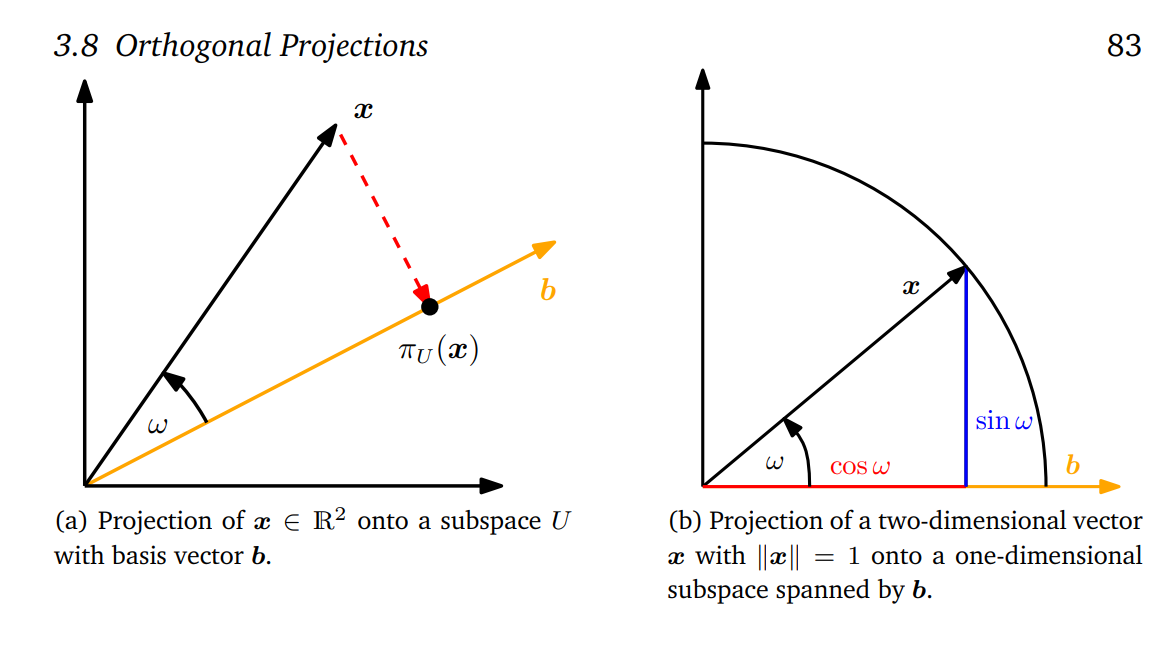
\includegraphics[width=0.6\textwidth]{./Images/Projection onto a line.png}
\end{center}

where \(x\) is projected onto a one-dimensional subspace \(U\subseteq\mathbb{R}^n\) spanned by basis vector \(b\). This goes through the origin.

When projecting \(x \in \mathbb{R}^n\) onto \(U\), we want to find the vector \(\pi_U(X) \in U \) that is closest to x.

\begin{prop}
  
  As before we minimise \(||x-\pi_U(x)||^2\). This implies that \(x-\pi_U(x)\) is orthogonal to \(U\) and thus also orthogonal to the basis vector \(b\).
  \[\langle x-\pi_U(x),b \rangle = 0\]
\end{prop}

\begin{prop}
  Further, the projection \(\pi_U(x)\) must be an element of \(U\) and so is a scalar multiple of \(b\), which spans U. Hence: \[\pi_U(x)=\lambda b\] for some \(\lambda \in \mathbb{R}\)
\end{prop}

\subsection{Finding \(\lambda\)}

Substituting Prop 1.4.2 into 1.4.1 we get:
\[\langle x-\lambda b,b \rangle = 0\]

Exploiting the bilinearity of the inner product:
\[\langle x,b \rangle - \lambda \langle b,b \rangle = 0\]
\[\implies \lambda = \frac{\langle x,b \rangle}{\langle b,b \rangle} = \frac{\langle x,b \rangle}{ ||b||^2} = \frac{x'b}{b'b}\]

\subsection{Finding \(\pi_U(x)\)}

Since \(\pi_U(x)=\lambda b\), we have:
\[\pi_U(x)=\frac{x'b}{b'b}b\]

The length of \(\pi_U(x)\) is: \[||\pi_U(x)||=||\lambda b||=|\lambda| \hspace{0.5mm} ||b||\] Thus the projection acts as a coordinate of \(\pi_U(x)\) in the direction of \(b\).

Using the dot product as the inner product we have:
\[=\frac{|x'b|}{||b||^2}||b||=|cos(\theta)|\hspace{0.5mm}||x||\hspace{0.5mm}||b||\frac{||b||}{||b||^2}=|cos(\theta)|\hspace{0.5mm}||x||\]

\subsection{The Projection Matrix \(P_\pi\)}
As projection is a linear mapping, there exists a matrix \(P_\pi\) such that: \[\pi_U(x)=P_\pi x\]
With the dot as the inner product and \[\pi_U(x)=\lambda b = b\lambda = b\frac{b'x}{||b||^2}=\frac{bb'}{||b||^2}x\]
Thus \[P_\pi=\frac{bb'}{||b||^2}\]

\section{Projection Onto a General Subspace}
We find a projection of \(x \in \mathbb{R}^n\) onto a subspace \(U \subseteq \mathbb{R}^n\) with \(dim(U)=m\geq1\).
Assume that \(b_1,...,b_m\) is an ordered basis for \(U\). Any projection \(\pi_U(x)\) onto \(U\) can be written as a linear combination of the basis vectors: such that \(\pi_U(x)=\sum_{i=1}^{m}\lambda_i b_i\).
We follow the same three step procedure as before:

\subsection{Finding \(\lambda_1,...,\lambda_m\)}
We find coordinates \(\lambda_1,...,\lambda_m\) such that the linear combination
\[\pi_U(x)=\sum_{i=1}^{m}\lambda_i b_i=\bold{B}\vec{\lambda}\]
\[\bold{B}=\begin{bmatrix}
  \vec{b_1} & ... & \vec{b_m}
\end{bmatrix}, \in \mathbb{R}^{n\times m}, \vec{\lambda}=\begin{bmatrix}
  \lambda_1 \\ ... \\ \lambda_m
\end{bmatrix} \in \mathbb{R}^m\]
is such that \(\pi_U(x)\) is the closest point in \(U\) to \(x\). This implies that \(x-\pi_U(x)\) is orthogonal to \(U\) and thus also orthogonal to each basis vector \(b_i\). Thus we obtain simultaneous equations:
\[\langle x-\pi_U(x),b_1 \rangle = b_1'(x-\pi_U(x))=0\]
\[\vdots\]
\[\langle x-\pi_U(x),b_m \rangle = b_m'(x-\pi_U(x))=0\] 
as \(\pi_U(x)=\bold{B}\vec{\lambda}\) we have:
\[b_1'(x-\bold{B}\vec{\lambda})=0\]
\[\vdots\]
\[b_m'(x-\bold{B}\vec{\lambda})=0\]
thus we obtain a homogeneous system of linear equations:
\[\begin{bmatrix}
  b_1' \\ \vdots \\ b_m'
\end{bmatrix}(x-\bold{B}\vec{\lambda})=0\]
\[\iff \bold{B}'(x-\bold{B}\vec{\lambda})=0\]
\[\iff \bold{B}'\bold{B}\vec{\lambda}=\bold{B}'x\]
\[\iff \vec{\lambda}=(\bold{B}'\bold{B})^{-1}\bold{B}'x\]
where we require that \(\bold{B}'\bold{B}\) is invertible, which is true if and only if \(\bold{B}\) has full column rank, which is true if and only if the basis vectors \(b_1,...,b_m\) are linearly independent.

\subsection{Finding \(\pi_U(x)\)}
We have that \(\pi_U(x)=\bold{B}\vec{\lambda}\) and so:
\[\pi_U(x)=\bold{B}(\bold{B}'\bold{B})^{-1}\bold{B}'x\]

\subsection{The Projection Matrix \(P_\pi\)}
As projection is a linear mapping, there exists a matrix \(P_\pi\) such that: \[\pi_U(x)=P_\pi x\]
Thus \[P_\pi=\bold{B}(\bold{B}'\bold{B})^{-1}\bold{B}'\]

\section{Appendix: OLS Estimator Equivalence}

\begin{claim}
  \[\hat{\beta}=(X'X)^{-1}X'Y=\frac{\sum(X_i-\bar{X})(Y_i-\bar{Y})}{\sum(X_i-\bar{X})^2}\]
  \[\iff X\] includes a constant
\end{claim}

Let us take the case for \(k=1\), i.e. \(X\) is a vector of length \(n\). Then: suppose \(X\) includes a constant, i.e. \(X=\begin{bmatrix}
  1 & x_1 \\ \vdots & \vdots \\ 1 & x_n \end{bmatrix}\). Then let \(\tilde{x_i}=(1,x_i)'\) Then \(X= (\tilde{x_1},...,\tilde{x_n})'\)
Thus:
  \[(X'X)^{-1}X'Y = (\sum_{i=1}^{n}\tilde{x_i}\tilde{x_i}')^{-1}\sum_{i=1}^{n}\tilde{x_i}y_i\]
  \[=\left[\sum_{i=1}^{n}\begin{bmatrix}
    1 & x_i \\ x_i & x_i^2 \end{bmatrix}\right]^{-1}\sum_{i=1}^{n} \begin{bmatrix}
        1 \\ x_i \end{bmatrix}Y_i\]
  \[=\left[ n\begin{bmatrix}
    1 & \bar{x} \\ \bar{x} & \frac{1}{n}\sum_{i=1}^{n}x_i^2 \end{bmatrix}\right]^{-1} n\begin{bmatrix}
      \bar{y} \\ \frac{1}{n}\sum_{i=1}^{n}x_iy_i  \end{bmatrix}\]
      =\[\frac{1}{\frac{1}{n}\sum_{i=1}^{n}x_i^2-\bar{x}^2}\begin{bmatrix}
        \frac{1}{n}\sum_{i=1}^{n}x_i^2 & -\bar{x} \\ -\bar{x} & 1 \end{bmatrix} \begin{bmatrix}
          \bar{y} \\ \frac{1}{n}\sum_{i=1}^{n}x_iy_i  \end{bmatrix}\]
  
The second component is the estimate fo the slope coefficient, and the first component is the estimate of the intercept coefficient. Thus we have:
\[\hat{\beta}=\frac{\sum(X_i-\bar{X})(Y_i-\bar{Y})}{\sum(X_i-\bar{X})^2}\]

\end{document}